% Part 2: Agent Foundations & Concepts
% A Comprehensive Guide to Agentic Coding Tools
% University of South Carolina

\documentclass[aspectratio=169, 11pt]{beamer}

% ============================================
% Theme and Color Setup (UofSC Colors)
% ============================================
\usetheme{Madrid}
\usecolortheme{default}

% Define UofSC Colors
\definecolor{UofSCGarnet}{HTML}{73000a}
\definecolor{UofSCBlack}{HTML}{000000}
\definecolor{UofSCWhite}{HTML}{ffffff}
\definecolor{UofSCAtlantic}{HTML}{466A9F}
\definecolor{UofSCCongaree}{HTML}{1F414D}
\definecolor{UofSCRose}{HTML}{CC2E40}
\definecolor{UofSCHorseshoe}{HTML}{65780B}
\definecolor{UofSCGrass}{HTML}{CED318}
\definecolor{UofSCHoneycomb}{HTML}{A49137}
\definecolor{UofSCDarkGarnet}{HTML}{570008}
\definecolor{UofSCAzalea}{HTML}{844247}
\definecolor{UofSC90Black}{HTML}{363636}
\definecolor{UofSC70Black}{HTML}{5C5C5C}
\definecolor{UofSC50Black}{HTML}{A2A2A2}
\definecolor{UofSCWarmGrey}{HTML}{676156}
\definecolor{UofSCSandstorm}{HTML}{FFF2E3}

% Apply UofSC colors to beamer elements
\setbeamercolor{palette primary}{bg=UofSCGarnet, fg=UofSCWhite}
\setbeamercolor{palette secondary}{bg=UofSCCongaree, fg=UofSCWhite}
\setbeamercolor{palette tertiary}{bg=UofSCAtlantic, fg=UofSCWhite}
\setbeamercolor{palette quaternary}{bg=UofSCBlack, fg=UofSCWhite}
\setbeamercolor{structure}{fg=UofSCGarnet}
\setbeamercolor{section in toc}{fg=UofSCBlack}
\setbeamercolor{subsection in toc}{fg=UofSCCongaree}
\setbeamercolor{title}{fg=UofSCWhite, bg=UofSCGarnet}
\setbeamercolor{frametitle}{fg=UofSCWhite, bg=UofSCGarnet}
\setbeamercolor{block title}{bg=UofSCGarnet, fg=UofSCWhite}
\setbeamercolor{block body}{bg=UofSCSandstorm, fg=UofSCBlack}
\setbeamercolor{block title alerted}{bg=UofSCRose, fg=UofSCWhite}
\setbeamercolor{block body alerted}{bg=UofSCSandstorm, fg=UofSCBlack}
\setbeamercolor{block title example}{bg=UofSCAtlantic, fg=UofSCWhite}
\setbeamercolor{block body example}{bg=UofSCSandstorm, fg=UofSCBlack}
\setbeamercolor{itemize item}{fg=UofSCGarnet}
\setbeamercolor{itemize subitem}{fg=UofSCCongaree}
\setbeamercolor{enumerate item}{fg=UofSCGarnet}
\setbeamercolor{enumerate subitem}{fg=UofSCCongaree}

% Remove rounded corners (sharp edges only)
\setbeamertemplate{blocks}[default]
\setbeamertemplate{title page}[default]
\setbeamertemplate{itemize items}[square]
\setbeamertemplate{enumerate items}[default]

% Remove navigation symbols
\setbeamertemplate{navigation symbols}{}

% Add frame numbers
\setbeamertemplate{footline}{
  \hfill
  \usebeamercolor[fg]{page number in head/foot}
  \usebeamerfont{page number in head/foot}
  \insertframenumber\,/\,\inserttotalframenumber\kern1em\vskip2pt
}

% ============================================
% Required Packages
% ============================================
\usepackage{tikz}
\usetikzlibrary{shapes.geometric, arrows.meta, positioning, fit, calc, backgrounds}
\usepackage{listings}
\usepackage{amsmath}
\usepackage{amssymb}
\usepackage{fontawesome5}
\usepackage{booktabs}
\usepackage{xcolor}
\usepackage{hyperref}

% ============================================
% TikZ Styles
% ============================================
\tikzset{
    % Box styles with sharp corners
    component/.style={
        rectangle,
        draw=UofSCBlack,
        fill=UofSCWhite,
        thick,
        minimum width=3cm,
        minimum height=1cm,
        align=center,
        font=\small
    },
    component garnet/.style={
        component,
        fill=UofSCGarnet!10,
        draw=UofSCGarnet,
        thick
    },
    component atlantic/.style={
        component,
        fill=UofSCAtlantic!10,
        draw=UofSCAtlantic,
        thick
    },
    component congaree/.style={
        component,
        fill=UofSCCongaree!10,
        draw=UofSCCongaree,
        thick
    },
    loop node/.style={
        rectangle,
        draw=UofSCGarnet,
        fill=UofSCGarnet!15,
        thick,
        minimum width=2.5cm,
        minimum height=1.2cm,
        align=center,
        font=\footnotesize\bfseries
    },
    decision/.style={
        diamond,
        draw=UofSCBlack,
        fill=UofSCHoneycomb!20,
        thick,
        minimum width=2cm,
        minimum height=1.5cm,
        align=center,
        font=\footnotesize,
        aspect=2
    },
    arrow style/.style={
        ->,
        >=Stealth,
        thick,
        UofSCBlack
    },
    biarrow style/.style={
        <->,
        >=Stealth,
        thick,
        UofSCBlack
    }
}

% ============================================
% Code Listing Style
% ============================================
\lstset{
    basicstyle=\ttfamily\scriptsize,
    backgroundcolor=\color{UofSCSandstorm},
    frame=single,
    framerule=0.5pt,
    rulecolor=\color{UofSCBlack},
    numbers=left,
    numberstyle=\tiny\color{UofSC70Black},
    numbersep=5pt,
    breaklines=true,
    showstringspaces=false,
    keywordstyle=\color{UofSCGarnet}\bfseries,
    commentstyle=\color{UofSCHorseshoe}\itshape,
    stringstyle=\color{UofSCAtlantic},
    tabsize=2
}

% ============================================
% Title Information
% ============================================
\title[Part 2: Agent Foundations]{Part 2: Agent Foundations \& Concepts}
\subtitle{Understanding the Foundation of Agentic Coding Tools}
\author{Agentic Coding Tools Series}
\institute{University of South Carolina}
\date{\today}

% ============================================
% Document Begin
% ============================================
\begin{document}

% --------------------------------------------
% Title Slide
% --------------------------------------------
\begin{frame}[plain]
    \titlepage
\end{frame}

% --------------------------------------------
% Table of Contents
% --------------------------------------------
\begin{frame}{Overview}
    \tableofcontents
\end{frame}

% ============================================
% SECTION 1: What IS an Agent?
% ============================================
\section{What IS an Agent?}

% --------------------------------------------
\begin{frame}{Formal Definition: What is an Agent?}
    \begin{columns}[T]
        \begin{column}{0.5\textwidth}
            \textbf{An agent is an autonomous software system that:}
            \begin{enumerate}
                \item \textbf{Perceives} its environment through sensors/tools
                \item \textbf{Reasons} about the current state and goals
                \item \textbf{Takes Actions} to influence the environment
                \item \textbf{Observes} the results of those actions
                \item \textbf{Adapts} behavior based on feedback
            \end{enumerate}
        \end{column}
        \begin{column}{0.5\textwidth}
            \begin{block}{Mathematical Definition}
                \centering
                Agent $= \langle P, S, A, \delta, \gamma, G \rangle$
                \vspace{0.3cm}
                \begin{tabular}{ll}
                    $P$ & Perception (observations) \\
                    $S$ & State space \\
                    $A$ & Action space \\
                    $\delta$ & State transition function \\
                    $\gamma$ & Goal evaluation function \\
                    $G$ & Goal specification \\
                \end{tabular}
            \end{block}
        \end{column}
    \end{columns}

    \note{This formal definition comes from classical AI theory (Russell \& Norvig). The key insight is that an agent is not just reactive---it perceives, reasons about what it perceives, takes actions based on reasoning, and then observes outcomes.}
\end{frame}

% --------------------------------------------
\begin{frame}{Agent vs Traditional AI Assistant}
    \begin{center}
    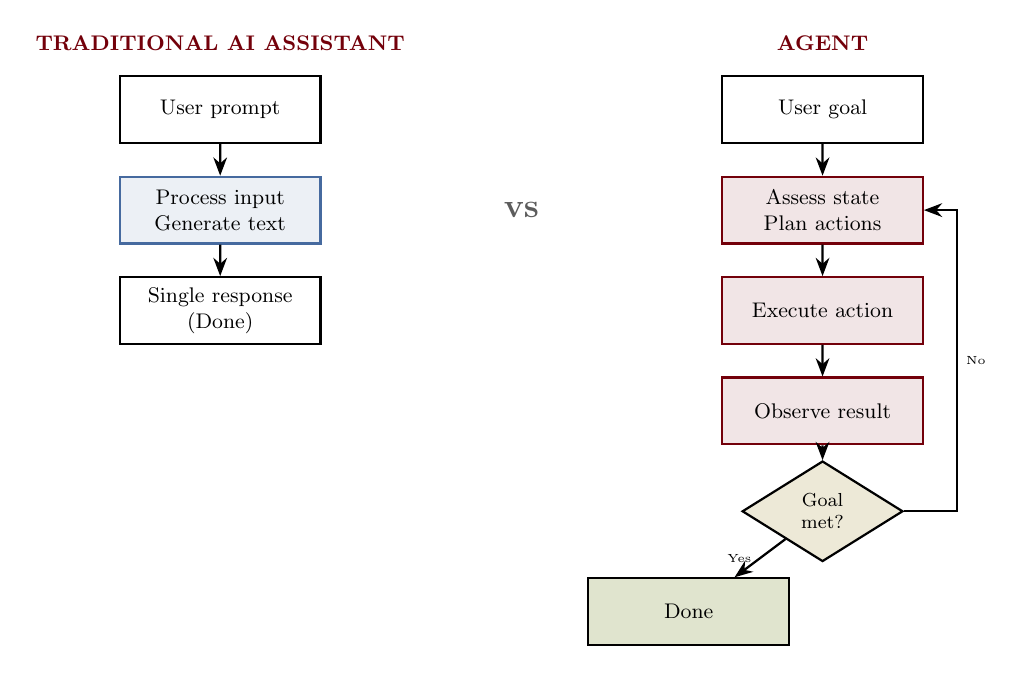
\begin{tikzpicture}[scale=0.85, transform shape]
        % Traditional AI Assistant (left side)
        \node[font=\small\bfseries, text=UofSCGarnet] at (-4.5, 4) {TRADITIONAL AI ASSISTANT};

        \node[component] (trad-input) at (-4.5, 3) {User prompt};
        \node[component atlantic] (trad-process) at (-4.5, 1.5) {Process input\\Generate text};
        \node[component] (trad-output) at (-4.5, 0) {Single response\\(Done)};

        \draw[arrow style] (trad-input) -- (trad-process);
        \draw[arrow style] (trad-process) -- (trad-output);

        % VS
        \node[font=\Large\bfseries, text=UofSC70Black] at (0, 1.5) {vs};

        % Agent (right side)
        \node[font=\small\bfseries, text=UofSCGarnet] at (4.5, 4) {AGENT};

        \node[component] (agent-input) at (4.5, 3) {User goal};
        \node[component garnet] (agent-assess) at (4.5, 1.5) {Assess state\\Plan actions};
        \node[component garnet] (agent-execute) at (4.5, 0) {Execute action};
        \node[component garnet] (agent-observe) at (4.5, -1.5) {Observe result};
        \node[decision] (agent-decision) at (4.5, -3) {Goal\\met?};
        \node[component, fill=UofSCHorseshoe!20] (agent-done) at (2.5, -4.5) {Done};

        \draw[arrow style] (agent-input) -- (agent-assess);
        \draw[arrow style] (agent-assess) -- (agent-execute);
        \draw[arrow style] (agent-execute) -- (agent-observe);
        \draw[arrow style] (agent-observe) -- (agent-decision);
        \draw[arrow style] (agent-decision) -- node[left, font=\tiny] {Yes} (agent-done);
        \draw[arrow style] (agent-decision.east) -- ++(0.8,0) |- node[right, font=\tiny, pos=0.25] {No} (agent-assess.east);
    \end{tikzpicture}
    \end{center}

    \note{The fundamental difference is autonomy and iteration. A traditional AI assistant is stateless. An agent is stateful and goal-directed---it operates in a loop.}
\end{frame}

% --------------------------------------------
\begin{frame}{Key Characteristics of Agents}
    \begin{columns}[T]
        \begin{column}{0.33\textwidth}
            \begin{block}{\#1 Autonomy}
                The ability to make decisions and take actions without constant user direction
                \vspace{0.3cm}

                \textbf{Spectrum:}
                \begin{itemize}
                    \item Manual (Chatbot)
                    \item Semi-Autonomous
                    \item Fully Autonomous
                \end{itemize}
            \end{block}
        \end{column}
        \begin{column}{0.33\textwidth}
            \begin{block}{\#2 Goal-Directed}
                Behavior determined by explicit objectives, not instructions
                \vspace{0.3cm}

                \textbf{Example:}
                \begin{itemize}
                    \item ``Minimize test runtime to under 100ms''
                    \item Agent finds its own approach
                \end{itemize}
            \end{block}
        \end{column}
        \begin{column}{0.33\textwidth}
            \begin{block}{\#3 Tool Use}
                Agents act on environments through well-defined tools
                \vspace{0.3cm}

                \textbf{Without tools:} \\
                Agent can only think

                \textbf{With tools:} \\
                Agent can think AND do
            \end{block}
        \end{column}
    \end{columns}

    \note{Most practical agents operate in the ``Semi-Autonomous'' zone where they can execute a series of steps but are bounded by explicit constraints and user confirmation checkpoints.}
\end{frame}

% --------------------------------------------
\begin{frame}{Why Agents Matter for Software Development}
    \begin{columns}[T]
        \begin{column}{0.45\textwidth}
            \textbf{Traditional Development:}
            \begin{itemize}
                \item Write code
                \item Run tests
                \item Fix errors
                \item Repeat
            \end{itemize}
            \textit{Human-intensive, one decision at a time}
        \end{column}
        \begin{column}{0.55\textwidth}
            \textbf{Agentic Development:}
            \begin{itemize}
                \item Agent: Implement feature
                \begin{itemize}
                    \item Write code
                    \item Run tests
                    \item Fix failures
                    \item Optimize performance
                    \item Add documentation
                    \item Submit for review
                \end{itemize}
            \end{itemize}
        \end{column}
    \end{columns}

    \vspace{0.5cm}
    \begin{block}{Benefits}
        \begin{itemize}
            \item Parallelizable tasks (agent explores while humans plan)
            \item Tedious tasks automated (debugging, testing)
            \item 24/7 availability and consistent process execution
        \end{itemize}
    \end{block}

    \note{Agents are particularly valuable for software development because code is deterministic and testable. Unlike domains with ambiguous feedback, code has clear pass/fail signals from tests.}
\end{frame}

% ============================================
% SECTION 2: Core Agent Components
% ============================================
\section{Core Agent Components}

% --------------------------------------------
\begin{frame}{Core Agent Components: The Architecture}
    \begin{center}
    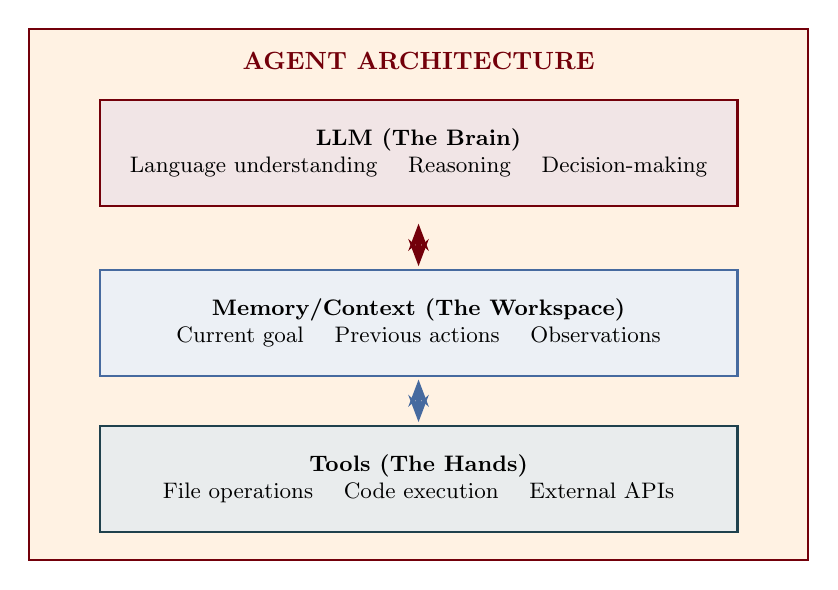
\begin{tikzpicture}[scale=0.9, transform shape]
        % Main container
        \node[draw=UofSCGarnet, thick, minimum width=11cm, minimum height=7.5cm, fill=UofSCSandstorm] (container) at (0,0) {};
        \node[font=\bfseries, text=UofSCGarnet] at (0, 3.3) {AGENT ARCHITECTURE};

        % LLM (Brain)
        \node[component garnet, minimum width=9cm, minimum height=1.5cm] (llm) at (0, 2) {
            \textbf{LLM (The Brain)}\\
            Language understanding \quad Reasoning \quad Decision-making
        };

        % Bidirectional arrow
        \draw[biarrow style, UofSCGarnet, line width=1.5pt] (0, 1) -- (0, 0.4);

        % Memory/Context
        \node[component atlantic, minimum width=9cm, minimum height=1.5cm] (memory) at (0, -0.4) {
            \textbf{Memory/Context (The Workspace)}\\
            Current goal \quad Previous actions \quad Observations
        };

        % Bidirectional arrow
        \draw[biarrow style, UofSCAtlantic, line width=1.5pt] (0, -1.2) -- (0, -1.8);

        % Tools
        \node[component congaree, minimum width=9cm, minimum height=1.5cm] (tools) at (0, -2.6) {
            \textbf{Tools (The Hands)}\\
            File operations \quad Code execution \quad External APIs
        };
    \end{tikzpicture}
    \end{center}

    \note{Think of an agent like a person at a desk. The LLM is their brain (thinking and reasoning). Memory/context is their workspace (what they're currently focused on). Tools are their hands (how they interact with the world).}
\end{frame}

% --------------------------------------------
\begin{frame}{Component \#1: The LLM --- The Brain}
    \begin{columns}[T]
        \begin{column}{0.5\textwidth}
            \begin{center}
            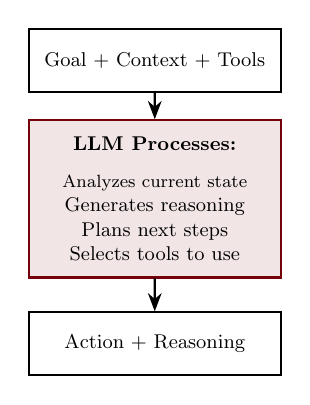
\begin{tikzpicture}[scale=0.8, transform shape]
                \node[component, minimum width=4cm] (input) at (0, 3) {Goal + Context + Tools};
                \node[component garnet, minimum width=4cm, minimum height=2.5cm] (llm) at (0, 0.8) {
                    \textbf{LLM Processes:}\\[0.2cm]
                    \footnotesize
                    Analyzes current state\\
                    Generates reasoning\\
                    Plans next steps\\
                    Selects tools to use
                };
                \node[component, minimum width=4cm] (output) at (0, -1.5) {Action + Reasoning};

                \draw[arrow style] (input) -- (llm);
                \draw[arrow style] (llm) -- (output);
            \end{tikzpicture}
            \end{center}
        \end{column}
        \begin{column}{0.5\textwidth}
            \textbf{LLM Characteristics That Matter:}
            \begin{itemize}
                \item Quality of reasoning
                \item Instruction-following ability
                \item Tool use capability
                \item Consistency (reliability)
                \item Speed vs capability tradeoff
            \end{itemize}

            \vspace{0.3cm}
            \begin{exampleblock}{Model Selection}
                \footnotesize
                \begin{tabular}{ll}
                    Routine coding & Claude Haiku \\
                    Complex tasks & Claude Opus \\
                    Cost-sensitive & Llama3 \\
                \end{tabular}
            \end{exampleblock}
        \end{column}
    \end{columns}

    \note{The LLM is the ``intelligence'' in the system. Modern agents typically use frontier models because the quality of reasoning directly determines agent success.}
\end{frame}

% --------------------------------------------
\begin{frame}{Component \#2: Memory \& Context --- The Workspace}
    \begin{columns}[T]
        \begin{column}{0.5\textwidth}
            \textbf{What Lives in Memory:}
            \begin{itemize}
                \item \textbf{Goal:} ``Implement pagination for user API''
                \item \textbf{Observations:} Current code structure, previous test results, errors encountered
                \item \textbf{Reasoning History:} Steps tried, why they failed/succeeded
                \item \textbf{Plan:} Next actions, fallback strategies
            \end{itemize}

            \vspace{0.3cm}
            \textbf{Key Insight:}\\
            Memory = Context window usage\\
            More memory = Better decisions\\
            But: Context is \textit{finite and expensive}
        \end{column}
        \begin{column}{0.5\textwidth}
            \begin{block}{Context Window Sizes (2026)}
                \footnotesize
                \begin{tabular}{lr}
                    Claude Opus 4.5 & 200K tokens \\
                    GPT-4 Turbo & 128K tokens \\
                    Claude Haiku & 200K tokens \\
                    Gemini Pro 1.5 & \textbf{1M tokens} \\
                \end{tabular}
            \end{block}

            \vspace{0.3cm}
            \textbf{Management Strategies:}
            \begin{enumerate}
                \item Summarization
                \item Archival to files
                \item Forgetting old context
                \item Compression
                \item Phasing tasks
            \end{enumerate}
        \end{column}
    \end{columns}

    \note{Memory in modern LLM agents is not stored in a database---it's the prompt itself. This is both a strength and a limitation.}
\end{frame}

% --------------------------------------------
\begin{frame}{Component \#3: Tools --- The Hands}
    \begin{center}
    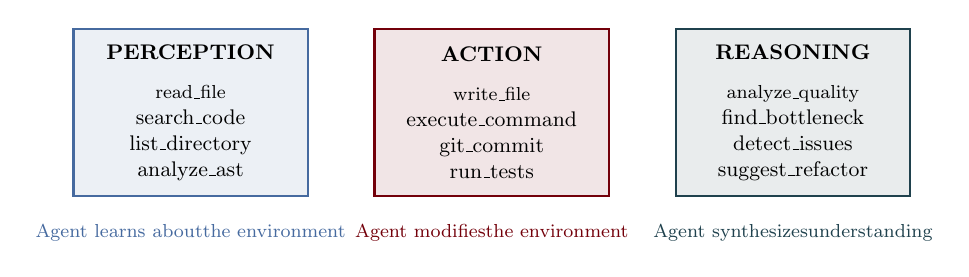
\begin{tikzpicture}[scale=0.85, transform shape]
        % Tool categories
        \node[component atlantic, minimum width=3.5cm, minimum height=2.5cm] (perception) at (-4.5, 0) {
            \textbf{PERCEPTION}\\[0.2cm]
            \footnotesize
            read\_file\\
            search\_code\\
            list\_directory\\
            analyze\_ast
        };

        \node[component garnet, minimum width=3.5cm, minimum height=2.5cm] (action) at (0, 0) {
            \textbf{ACTION}\\[0.2cm]
            \footnotesize
            write\_file\\
            execute\_command\\
            git\_commit\\
            run\_tests
        };

        \node[component congaree, minimum width=3.5cm, minimum height=2.5cm] (reasoning) at (4.5, 0) {
            \textbf{REASONING}\\[0.2cm]
            \footnotesize
            analyze\_quality\\
            find\_bottleneck\\
            detect\_issues\\
            suggest\_refactor
        };

        % Labels below
        \node[font=\footnotesize, text=UofSCAtlantic] at (-4.5, -1.8) {Agent learns about\\the environment};
        \node[font=\footnotesize, text=UofSCGarnet] at (0, -1.8) {Agent modifies\\the environment};
        \node[font=\footnotesize, text=UofSCCongaree] at (4.5, -1.8) {Agent synthesizes\\understanding};
    \end{tikzpicture}
    \end{center}

    \vspace{0.3cm}
    \begin{alertblock}{Tool Count Sweet Spot}
        \centering
        Too few (3--5): Agent paralyzed \quad\quad Optimal (8--15): Effective \quad\quad Too many (50+): Confused
    \end{alertblock}

    \note{Tool design is one of the most underestimated aspects of agent systems. Poor tools lead to agent confusion, failures, and hallucinations.}
\end{frame}

% --------------------------------------------
\begin{frame}{Component \#4: Planning Capability}
    \begin{columns}[T]
        \begin{column}{0.5\textwidth}
            \textbf{Non-Planning Agent:}
            \begin{enumerate}
                \item Read file
                \item Write changes
                \item Test
                \item Fails!
                \item Back to 1
                \item Loop 5 times...
            \end{enumerate}

            \textcolor{UofSCRose}{\textbf{Cost: High, Time: Long}}
        \end{column}
        \begin{column}{0.5\textwidth}
            \textbf{Planning Agent:}
            \begin{enumerate}
                \item \textbf{PLAN:}
                \begin{itemize}
                    \item Map structure
                    \item Identify patterns
                    \item Draft changes
                \end{itemize}
                \item Write smart
                \item Test
                \item Success!
            \end{enumerate}

            \textcolor{UofSCHorseshoe}{\textbf{Cost: Lower, Time: Shorter}}
        \end{column}
    \end{columns}

    \vspace{0.5cm}
    \begin{block}{Planning Techniques}
        \begin{itemize}
            \item \textbf{Hierarchical:} Break high-level goals into sub-tasks
            \item \textbf{Contingency:} IF condition THEN approach A ELSE approach B
            \item \textbf{Dependency:} Understand which changes affect which components
        \end{itemize}
    \end{block}

    \note{Planning separates good agents from bad ones. A planning agent thinks ``if I change X, it will affect Y, so I should also change Y.''}
\end{frame}

% ============================================
% SECTION 3: The ReAct Loop
% ============================================
\section{The ReAct Loop}

% --------------------------------------------
\begin{frame}{The ReAct Loop: Core Agent Operating Pattern}
    \begin{center}
    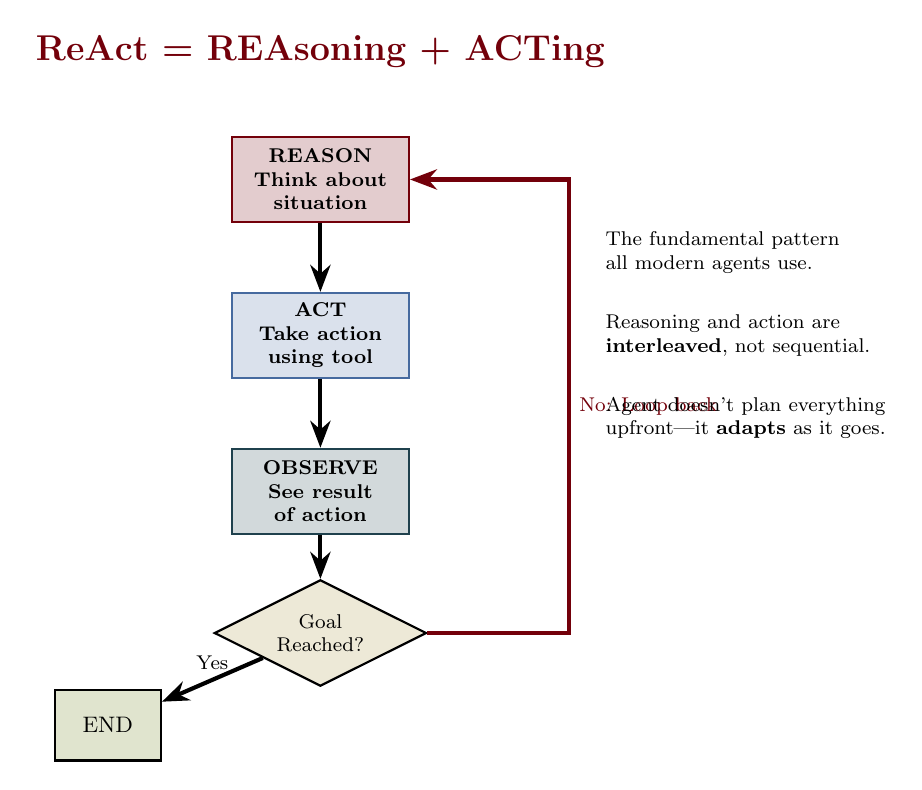
\begin{tikzpicture}[scale=0.9, transform shape]
        % Title
        \node[font=\Large\bfseries, text=UofSCGarnet] at (0, 4) {ReAct = REAsoning + ACTing};

        % REASON node
        \node[loop node, fill=UofSCGarnet!20] (reason) at (0, 2.2) {
            \textbf{REASON}\\
            Think about\\situation
        };

        % ACT node
        \node[loop node, fill=UofSCAtlantic!20, draw=UofSCAtlantic] (act) at (0, 0) {
            \textbf{ACT}\\
            Take action\\using tool
        };

        % OBSERVE node
        \node[loop node, fill=UofSCCongaree!20, draw=UofSCCongaree] (observe) at (0, -2.2) {
            \textbf{OBSERVE}\\
            See result\\of action
        };

        % Decision
        \node[decision, minimum width=2.5cm] (decision) at (0, -4.2) {Goal\\Reached?};

        % End node
        \node[component, fill=UofSCHorseshoe!20, minimum width=1.5cm] (end) at (-3, -5.5) {END};

        % Arrows
        \draw[arrow style, line width=1.5pt] (reason) -- (act);
        \draw[arrow style, line width=1.5pt] (act) -- (observe);
        \draw[arrow style, line width=1.5pt] (observe) -- (decision);
        \draw[arrow style, line width=1.5pt] (decision) -- node[above, font=\footnotesize] {Yes} (end);

        % Loop back arrow
        \draw[arrow style, line width=1.5pt, UofSCGarnet] (decision.east) -- ++(2,0) |- node[right, font=\footnotesize, pos=0.25] {No: Loop back} (reason.east);

        % Side explanation
        \node[align=left, font=\footnotesize] at (6, 0) {
            The fundamental pattern\\
            all modern agents use.\\[0.5cm]
            Reasoning and action are\\
            \textbf{interleaved}, not sequential.\\[0.5cm]
            Agent doesn't plan everything\\
            upfront---it \textbf{adapts} as it goes.
        };
    \end{tikzpicture}
    \end{center}

    \note{ReAct was formalized in a 2023 paper by Yao et al. The genius is that reasoning and action are interleaved, not sequential.}
\end{frame}

% --------------------------------------------
\begin{frame}{REASON Step: Thinking About the Situation}
    \begin{columns}[T]
        \begin{column}{0.5\textwidth}
            \textbf{Input to REASON:}
            \begin{itemize}
                \item Current goal: ``Fix failing tests in auth module''
                \item What we know so far:
                \begin{itemize}
                    \item Test failures from previous step
                    \item Code we've examined
                    \item Changes we've made
                \end{itemize}
                \item What we still need:
                \begin{itemize}
                    \item More information?
                    \item To take action?
                    \item To change something?
                \end{itemize}
            \end{itemize}
        \end{column}
        \begin{column}{0.5\textwidth}
            \begin{exampleblock}{LLM's Thinking Process}
                \footnotesize
                ``I see test X failed with error Y.
                The error looks like Z (connection refused).
                That suggests the database isn't running.
                I should check if database service is started.
                If not running, I'll start it.
                If running, I'll examine the connection string.''
            \end{exampleblock}

            \vspace{0.3cm}
            \textbf{Output of REASON:}
            \begin{itemize}
                \item Decision: What to do next
                \item Reasoning: Why that's right
                \item Expected outcome: What we'll learn
            \end{itemize}
        \end{column}
    \end{columns}

    \note{The REASON step is pure thought---no external effects. This is where agents can be brilliant or terrible depending on LLM quality.}
\end{frame}

% --------------------------------------------
\begin{frame}{ACT Step: Taking Action}
    \begin{center}
    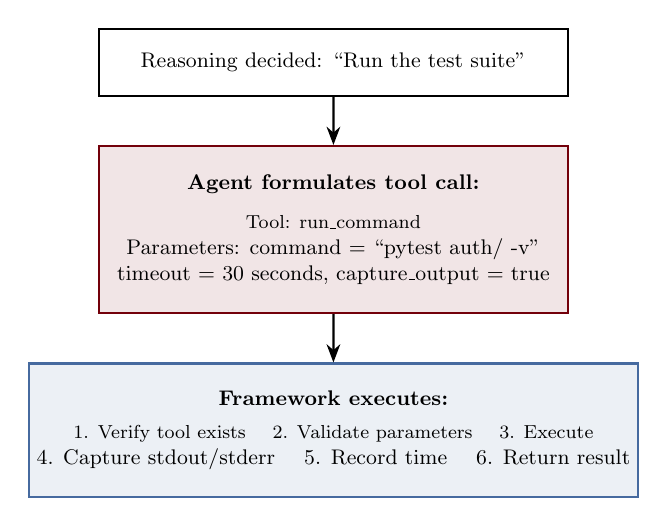
\begin{tikzpicture}[scale=0.85, transform shape]
        % Reasoning decided
        \node[component, minimum width=7cm] (decided) at (0, 3) {Reasoning decided: ``Run the test suite''};

        % Tool call box
        \node[component garnet, minimum width=7cm, minimum height=2.5cm] (toolcall) at (0, 0.5) {
            \textbf{Agent formulates tool call:}\\[0.2cm]
            \footnotesize
            Tool: run\_command\\
            Parameters: command = ``pytest auth/ -v''\\
            timeout = 30 seconds, capture\_output = true
        };

        % Framework execution
        \node[component atlantic, minimum width=7cm, minimum height=2cm] (framework) at (0, -2.5) {
            \textbf{Framework executes:}\\[0.1cm]
            \footnotesize
            1. Verify tool exists \quad 2. Validate parameters \quad 3. Execute\\
            4. Capture stdout/stderr \quad 5. Record time \quad 6. Return result
        };

        \draw[arrow style] (decided) -- (toolcall);
        \draw[arrow style] (toolcall) -- (framework);
    \end{tikzpicture}
    \end{center}

    \vspace{0.3cm}
    \begin{alertblock}{Key Insight}
        \centering
        \textbf{Action is the only step that changes the world}\\
        (everything else is thinking)
    \end{alertblock}

    \note{The LLM doesn't directly execute code---it decides what to execute and in what order. The framework handles actual execution and reporting.}
\end{frame}

% --------------------------------------------
\begin{frame}{OBSERVE Step: Perceiving Results}
    \begin{columns}[T]
        \begin{column}{0.55\textwidth}
            \begin{block}{System Output}
                \ttfamily\footnotesize
                \$ pytest auth/ -v\\[0.2cm]
                test\_login\_valid\_user ... PASS\\
                test\_login\_invalid\_user ... PASS\\
                test\_session\_timeout ... FAIL\\
                \quad AssertionError: Session not expired\\[0.2cm]
                2 passed, 1 failed in 2.34s
            \end{block}

            \vspace{0.3cm}
            \begin{exampleblock}{Agent's Observation}
                \footnotesize
                ``2 passed, 1 failed. The failure is in test\_session\_timeout and the message is `Session not expired'. This suggests the timeout logic isn't working.''
            \end{exampleblock}
        \end{column}
        \begin{column}{0.45\textwidth}
            \textbf{Good Observation includes:}
            \begin{itemize}
                \item[\textcolor{UofSCHorseshoe}{\checkmark}] What succeeded (2 tests passed)
                \item[\textcolor{UofSCHorseshoe}{\checkmark}] What failed (1 test failed)
                \item[\textcolor{UofSCHorseshoe}{\checkmark}] Why it failed (timeout not working)
                \item[\textcolor{UofSCHorseshoe}{\checkmark}] What to do next
            \end{itemize}

            \vspace{0.3cm}
            \textbf{Poor Observation:}
            \begin{itemize}
                \item[\textcolor{UofSCRose}{$\times$}] Just reports: ``Tests ran''
                \item[\textcolor{UofSCRose}{$\times$}] Misses details
                \item[\textcolor{UofSCRose}{$\times$}] Doesn't extract next step
            \end{itemize}
        \end{column}
    \end{columns}

    \note{The OBSERVE step is critical but often overlooked. It's not just about receiving output---it's about interpreting it correctly.}
\end{frame}

% --------------------------------------------
\begin{frame}{Complete ReAct Cycle: An Example}
    \begin{center}
    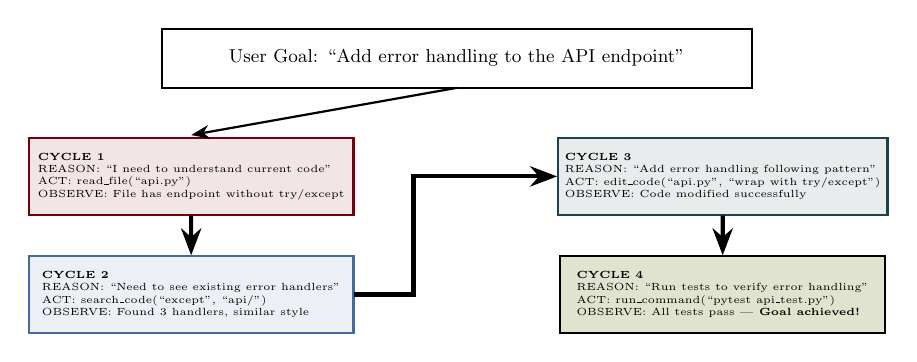
\begin{tikzpicture}[scale=0.75, transform shape]
        % Cycle 1
        \node[component garnet, minimum width=5.5cm, minimum height=1.3cm, align=left, font=\tiny] (c1) at (-4.5, 2.5) {
            \textbf{CYCLE 1}\\
            REASON: ``I need to understand current code''\\
            ACT: read\_file(``api.py'')\\
            OBSERVE: File has endpoint without try/except
        };

        % Cycle 2
        \node[component atlantic, minimum width=5.5cm, minimum height=1.3cm, align=left, font=\tiny] (c2) at (-4.5, 0.5) {
            \textbf{CYCLE 2}\\
            REASON: ``Need to see existing error handlers''\\
            ACT: search\_code(``except'', ``api/'')\\
            OBSERVE: Found 3 handlers, similar style
        };

        % Cycle 3
        \node[component congaree, minimum width=5.5cm, minimum height=1.3cm, align=left, font=\tiny] (c3) at (4.5, 2.5) {
            \textbf{CYCLE 3}\\
            REASON: ``Add error handling following pattern''\\
            ACT: edit\_code(``api.py'', ``wrap with try/except'')\\
            OBSERVE: Code modified successfully
        };

        % Cycle 4
        \node[component, fill=UofSCHorseshoe!20, minimum width=5.5cm, minimum height=1.3cm, align=left, font=\tiny] (c4) at (4.5, 0.5) {
            \textbf{CYCLE 4}\\
            REASON: ``Run tests to verify error handling''\\
            ACT: run\_command(``pytest api\_test.py'')\\
            OBSERVE: All tests pass --- \textbf{Goal achieved!}
        };

        % Arrows
        \draw[arrow style, line width=1.5pt] (c1) -- (c2);
        \draw[arrow style, line width=1.5pt] (c2.east) -- ++(1,0) |- (c3.west);
        \draw[arrow style, line width=1.5pt] (c3) -- (c4);

        % User goal at top
        \node[component, minimum width=10cm] at (0, 4.5) {User Goal: ``Add error handling to the API endpoint''};
        \draw[arrow style] (0, 4) -- (-4.5, 3.2);
    \end{tikzpicture}
    \end{center}

    \note{Notice how each cycle informs the next. The agent learns something in OBSERVE that shapes what it REASONS about next. This is fundamentally different from waterfall planning.}
\end{frame}

% --------------------------------------------
\begin{frame}{Why ReAct Works: Comparison}
    \begin{center}
    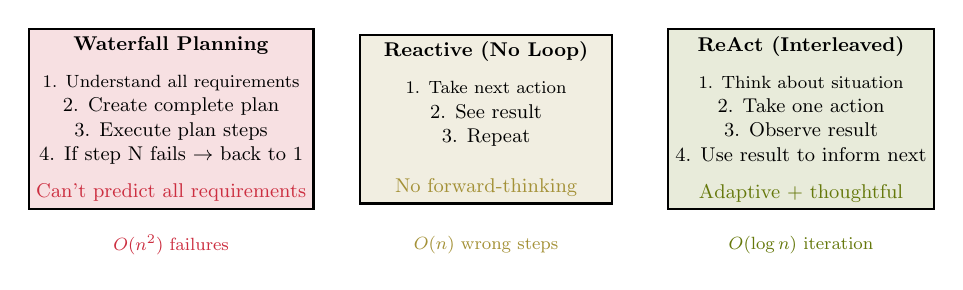
\begin{tikzpicture}[scale=0.8, transform shape]
        % Waterfall
        \node[component, minimum width=4cm, minimum height=2.5cm, fill=UofSCRose!15] (waterfall) at (-5, 0) {
            \textbf{Waterfall Planning}\\[0.2cm]
            \footnotesize
            1. Understand all requirements\\
            2. Create complete plan\\
            3. Execute plan steps\\
            4. If step N fails $\rightarrow$ back to 1\\[0.2cm]
            \textcolor{UofSCRose}{Can't predict all requirements}
        };

        % Reactive
        \node[component, minimum width=4cm, minimum height=2.5cm, fill=UofSCHoneycomb!15] (reactive) at (0, 0) {
            \textbf{Reactive (No Loop)}\\[0.2cm]
            \footnotesize
            1. Take next action\\
            2. See result\\
            3. Repeat\\[0.4cm]
            \textcolor{UofSCHoneycomb}{No forward-thinking}
        };

        % ReAct
        \node[component, minimum width=4cm, minimum height=2.5cm, fill=UofSCHorseshoe!15] (react) at (5, 0) {
            \textbf{ReAct (Interleaved)}\\[0.2cm]
            \footnotesize
            1. Think about situation\\
            2. Take one action\\
            3. Observe result\\
            4. Use result to inform next\\[0.2cm]
            \textcolor{UofSCHorseshoe}{Adaptive + thoughtful}
        };

        % Complexity labels below
        \node[font=\footnotesize, text=UofSCRose] at (-5, -2) {$O(n^2)$ failures};
        \node[font=\footnotesize, text=UofSCHoneycomb] at (0, -2) {$O(n)$ wrong steps};
        \node[font=\footnotesize, text=UofSCHorseshoe] at (5, -2) {$O(\log n)$ iteration};
    \end{tikzpicture}
    \end{center}

    \vspace{0.3cm}
    \begin{block}{ReAct Advantage}
        By making one change, observing the result, and using that observation to inform the next decision, agents avoid the cascading failures of pure planning.
    \end{block}

    \note{ReAct has become the dominant pattern because it's responsive to feedback. It's not about being smart at planning---it's about being responsive to feedback.}
\end{frame}

% ============================================
% SECTION 4: Agent Specialization
% ============================================
\section{Agent Specialization}

% --------------------------------------------
\begin{frame}{Generalists vs Specialists}
    \begin{columns}[T]
        \begin{column}{0.5\textwidth}
            \begin{block}{Generalist Agent}
                ``Do whatever task is needed''
                \vspace{0.2cm}

                \textbf{Can handle:} Coding, Testing, Deployment, Documentation

                \vspace{0.2cm}
                \textbf{Problems:}
                \begin{itemize}
                    \item[\textcolor{UofSCRose}{$\times$}] Slower (tries many approaches)
                    \item[\textcolor{UofSCRose}{$\times$}] Less accurate
                    \item[\textcolor{UofSCRose}{$\times$}] Context bloat
                    \item[\textcolor{UofSCRose}{$\times$}] Hard to debug
                \end{itemize}
            \end{block}
        \end{column}
        \begin{column}{0.5\textwidth}
            \begin{exampleblock}{Specialist Agent}
                ``Write Python tests for this code''
                \vspace{0.2cm}

                \textbf{Specialized for:} One language/framework, one type of task

                \vspace{0.2cm}
                \textbf{Advantages:}
                \begin{itemize}
                    \item[\textcolor{UofSCHorseshoe}{\checkmark}] Fast (fewer options)
                    \item[\textcolor{UofSCHorseshoe}{\checkmark}] Accurate (deep expertise)
                    \item[\textcolor{UofSCHorseshoe}{\checkmark}] Lean context
                    \item[\textcolor{UofSCHorseshoe}{\checkmark}] Easy to debug
                \end{itemize}
            \end{exampleblock}
        \end{column}
    \end{columns}

    \vspace{0.5cm}
    \begin{alertblock}{Modern Best Practice}
        \centering
        Use \textbf{multiple specialists + coordinator} instead of one generalist
    \end{alertblock}

    \note{A test-writing specialist will outperform a general agent at writing tests because it has test-specific tools and context.}
\end{frame}

% --------------------------------------------
\begin{frame}{Common Specialist Agent Types}
    \begin{center}
    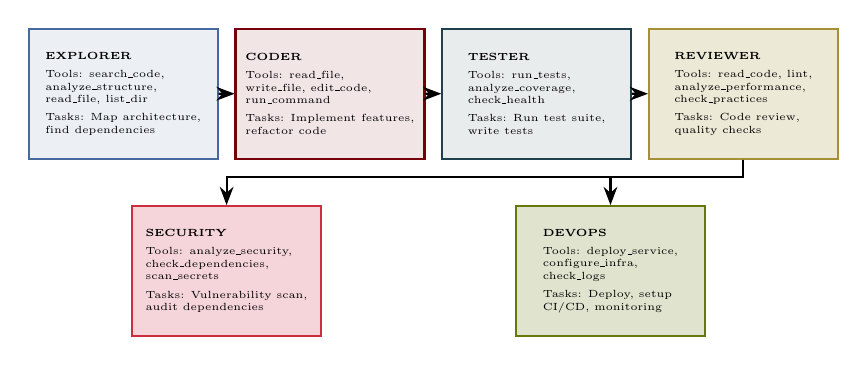
\begin{tikzpicture}[scale=0.75, transform shape]
        % Explorer
        \node[component atlantic, minimum width=3.2cm, minimum height=2.2cm, align=left, font=\tiny] (explorer) at (-5, 1.5) {
            \textbf{EXPLORER}\\[0.1cm]
            Tools: search\_code,\\
            analyze\_structure,\\
            read\_file, list\_dir\\[0.1cm]
            Tasks: Map architecture,\\
            find dependencies
        };

        % Coder
        \node[component garnet, minimum width=3.2cm, minimum height=2.2cm, align=left, font=\tiny] (coder) at (-1.5, 1.5) {
            \textbf{CODER}\\[0.1cm]
            Tools: read\_file,\\
            write\_file, edit\_code,\\
            run\_command\\[0.1cm]
            Tasks: Implement features,\\
            refactor code
        };

        % Tester
        \node[component congaree, minimum width=3.2cm, minimum height=2.2cm, align=left, font=\tiny] (tester) at (2, 1.5) {
            \textbf{TESTER}\\[0.1cm]
            Tools: run\_tests,\\
            analyze\_coverage,\\
            check\_health\\[0.1cm]
            Tasks: Run test suite,\\
            write tests
        };

        % Reviewer
        \node[component, fill=UofSCHoneycomb!20, draw=UofSCHoneycomb, minimum width=3.2cm, minimum height=2.2cm, align=left, font=\tiny] (reviewer) at (5.5, 1.5) {
            \textbf{REVIEWER}\\[0.1cm]
            Tools: read\_code, lint,\\
            analyze\_performance,\\
            check\_practices\\[0.1cm]
            Tasks: Code review,\\
            quality checks
        };

        % Security
        \node[component, fill=UofSCRose!20, draw=UofSCRose, minimum width=3.2cm, minimum height=2.2cm, align=left, font=\tiny] (security) at (-3.25, -1.5) {
            \textbf{SECURITY}\\[0.1cm]
            Tools: analyze\_security,\\
            check\_dependencies,\\
            scan\_secrets\\[0.1cm]
            Tasks: Vulnerability scan,\\
            audit dependencies
        };

        % DevOps
        \node[component, fill=UofSCHorseshoe!20, draw=UofSCHorseshoe, minimum width=3.2cm, minimum height=2.2cm, align=left, font=\tiny] (devops) at (3.25, -1.5) {
            \textbf{DEVOPS}\\[0.1cm]
            Tools: deploy\_service,\\
            configure\_infra,\\
            check\_logs\\[0.1cm]
            Tasks: Deploy, setup\\
            CI/CD, monitoring
        };

        % Pipeline arrows
        \draw[arrow style] (explorer) -- (coder);
        \draw[arrow style] (coder) -- (tester);
        \draw[arrow style] (tester) -- (reviewer);
        \draw[arrow style] (reviewer.south) -- ++(0,-0.3) -| (security.north);
        \draw[arrow style] (reviewer.south) -- ++(0,-0.3) -| (devops.north);
    \end{tikzpicture}
    \end{center}

    \note{Specialists are arranged in a pipeline. Explorer gathers information, Coder uses it to make changes. Neither does everything. This prevents bugs and allows parallelization.}
\end{frame}

% --------------------------------------------
\begin{frame}{Design Principles for Custom Specialists}
    \begin{enumerate}
        \item \textbf{Define Clear Responsibility}
        \begin{itemize}
            \item Specialist does ONE thing really well
            \item NOT: ``Handle all database operations''
            \item YES: ``Write SQL queries for this specific schema''
        \end{itemize}

        \item \textbf{Specify Exact Tools}
        \begin{itemize}
            \item Only the tools needed for this role
            \item NOT: ``Use all tools'' \quad YES: ``Use these 5 tools''
        \end{itemize}

        \item \textbf{Create Specialized Prompt}
        \begin{itemize}
            \item ``You are an expert in PostgreSQL. Your role is to write optimal queries...''
            \item Include domain-specific best practices
        \end{itemize}

        \item \textbf{Test Against Known Tasks}
        \begin{itemize}
            \item Verify specialist works on typical tasks
            \item ``Write query for active users'', ``Optimize slow report query''
        \end{itemize}
    \end{enumerate}

    \vspace{0.3cm}
    \begin{block}{Key Principles}
        Narrow is better than broad \quad\quad Specialization reduces error rate \quad\quad Prompts should be detailed
    \end{block}

    \note{The pattern is: focus the agent on one thing, give it the exact tools it needs, and prompt it to be expert in that area.}
\end{frame}

% ============================================
% SECTION 5: Context Windows Deep Dive
% ============================================
\section{Context Windows Deep Dive}

% --------------------------------------------
\begin{frame}{Context Windows: The Technical Foundation}
    \begin{columns}[T]
        \begin{column}{0.55\textwidth}
            \begin{center}
            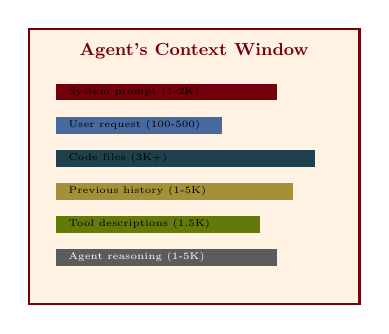
\begin{tikzpicture}[scale=0.7, transform shape]
                % Context window box
                \node[draw=UofSCGarnet, thick, minimum width=6cm, minimum height=5cm, fill=UofSCSandstorm] (window) at (0,0) {};
                \node[font=\small\bfseries, text=UofSCGarnet] at (0, 2.1) {Agent's Context Window};

                % Content bars
                \fill[UofSCGarnet] (-2.5, 1.5) rectangle (1.5, 1.2);
                \node[font=\tiny, anchor=west] at (-2.4, 1.35) {System prompt (1-2K)};

                \fill[UofSCAtlantic] (-2.5, 0.9) rectangle (0.5, 0.6);
                \node[font=\tiny, anchor=west] at (-2.4, 0.75) {User request (100-500)};

                \fill[UofSCCongaree] (-2.5, 0.3) rectangle (2.2, 0);
                \node[font=\tiny, anchor=west] at (-2.4, 0.15) {Code files (3K+)};

                \fill[UofSCHoneycomb] (-2.5, -0.3) rectangle (1.8, -0.6);
                \node[font=\tiny, anchor=west] at (-2.4, -0.45) {Previous history (1-5K)};

                \fill[UofSCHorseshoe] (-2.5, -0.9) rectangle (1.2, -1.2);
                \node[font=\tiny, anchor=west] at (-2.4, -1.05) {Tool descriptions (1.5K)};

                \fill[UofSC70Black] (-2.5, -1.5) rectangle (1.5, -1.8);
                \node[font=\tiny, anchor=west, text=white] at (-2.4, -1.65) {Agent reasoning (1-5K)};
            \end{tikzpicture}
            \end{center}
        \end{column}
        \begin{column}{0.45\textwidth}
            \textbf{What are Tokens?}
            \begin{itemize}
                \item 1 token $\approx$ 0.75 words (English)
                \item 1 token $\approx$ 4 characters
                \item 1 page $\approx$ 500--800 tokens
            \end{itemize}

            \vspace{0.3cm}
            \begin{block}{Window Size by Model (2026)}
                \footnotesize
                \begin{tabular}{lr}
                    Claude Haiku & 200K \\
                    Claude Opus 4.5 & 200K \\
                    GPT-4 Turbo & 128K \\
                    \textbf{Gemini Pro 1.5} & \textbf{1M} \\
                \end{tabular}
            \end{block}

            \vspace{0.2cm}
            \textcolor{UofSCGarnet}{\textbf{200K tokens $\approx$ 150 pages}}
        \end{column}
    \end{columns}

    \note{A 200K token context might sound huge, but a realistic task quickly consumes it. Understanding this limit is critical for effective agent design.}
\end{frame}

% --------------------------------------------
\begin{frame}{Token Limits: Theory vs Practice}
    \begin{columns}[T]
        \begin{column}{0.5\textwidth}
            \textbf{Theoretical:}
            \begin{itemize}
                \item Claude Opus: 200K tokens capacity
                \item = 150 pages of text
                \item ``Should be enough for any task''
            \end{itemize}

            \vspace{0.3cm}
            \textbf{Practical Consumption:}
            \begin{itemize}
                \item System prompt: 2K tokens
                \item Goal specification: 1K tokens
                \item Code files: 20K tokens
                \item Tool descriptions: 2K tokens
                \item Conversation history: 10K tokens
            \end{itemize}

            \textit{= 35K tokens before agent even starts working!}
        \end{column}
        \begin{column}{0.5\textwidth}
            \textbf{Agent reasoning consumes space:}
            \begin{itemize}
                \item Each decision: 500--2K tokens
                \item Each observation: 1K--5K tokens
                \item 10 cycles: $\sim$30K tokens
            \end{itemize}

            \vspace{0.3cm}
            \begin{alertblock}{Practical Rule of Thumb}
                Use no more than \textbf{50\%} of context window for ``setup'' (prompts, files, history)

                \vspace{0.2cm}
                If using $>$80\%, agent will run out of space mid-task and fail
            \end{alertblock}
        \end{column}
    \end{columns}

    \note{This is where many agent projects fail. Engineers think ``200K tokens is huge'' and load everything into context. Then the agent runs out of tokens mid-task.}
\end{frame}

% --------------------------------------------
\begin{frame}{Context Isolation: Multi-Agent Architecture}
    \begin{center}
    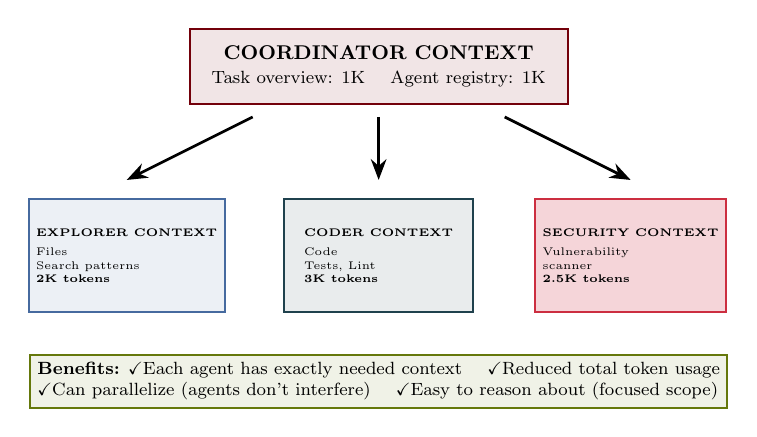
\begin{tikzpicture}[scale=0.8, transform shape]
        % Coordinator at top
        \node[component garnet, minimum width=6cm, minimum height=1.2cm] (coordinator) at (0, 3) {
            \textbf{COORDINATOR CONTEXT}\\
            \footnotesize Task overview: 1K \quad Agent registry: 1K
        };

        % Connection lines
        \draw[arrow style, line width=1pt] (-2, 2.2) -- (-4, 1.2);
        \draw[arrow style, line width=1pt] (0, 2.2) -- (0, 1.2);
        \draw[arrow style, line width=1pt] (2, 2.2) -- (4, 1.2);

        % Specialist agents
        \node[component atlantic, minimum width=3cm, minimum height=1.8cm, font=\tiny, align=left] (explorer) at (-4, 0) {
            \textbf{EXPLORER CONTEXT}\\[0.1cm]
            Files\\
            Search patterns\\
            \textbf{2K tokens}
        };

        \node[component congaree, minimum width=3cm, minimum height=1.8cm, font=\tiny, align=left] (coder) at (0, 0) {
            \textbf{CODER CONTEXT}\\[0.1cm]
            Code\\
            Tests, Lint\\
            \textbf{3K tokens}
        };

        \node[component, fill=UofSCRose!20, draw=UofSCRose, minimum width=3cm, minimum height=1.8cm, font=\tiny, align=left] (security) at (4, 0) {
            \textbf{SECURITY CONTEXT}\\[0.1cm]
            Vulnerability\\
            scanner\\
            \textbf{2.5K tokens}
        };

        % Benefits box
        \node[draw=UofSCHorseshoe, thick, fill=UofSCHorseshoe!10, minimum width=10cm, align=left, font=\footnotesize] (benefits) at (0, -2) {
            \textbf{Benefits:} \checkmark Each agent has exactly needed context \quad \checkmark Reduced total token usage\\
            \checkmark Can parallelize (agents don't interfere) \quad \checkmark Easy to reason about (focused scope)
        };
    \end{tikzpicture}
    \end{center}

    \note{When agents have isolated contexts, they can work in parallel and don't interfere with each other. The coordinator maintains minimal context and routes tasks to appropriate specialists.}
\end{frame}

% --------------------------------------------
\begin{frame}{Context Management Strategies}
    \begin{columns}[T]
        \begin{column}{0.5\textwidth}
            \textbf{Strategy 1: Chunking}
            \begin{itemize}
                \item Load only relevant file at a time
                \item Cycle 1: Load user\_routes.py, refactor, test, save
                \item Cycle 2: Load auth\_routes.py, refactor, test, save
                \item Cleaner, parallelizable
            \end{itemize}

            \vspace{0.3cm}
            \textbf{Strategy 2: Summarization}
            \begin{itemize}
                \item 10K-token class $\rightarrow$ 1K summary
                \item Keep method signatures, drop implementation details
                \item Saves 9K tokens
            \end{itemize}
        \end{column}
        \begin{column}{0.5\textwidth}
            \textbf{Strategy 3: Phasing}
            \begin{itemize}
                \item Phase 1: ``Fix critical bugs''
                \item Phase 2: ``Add type hints''
                \item Phase 3: ``Optimize performance''
                \item Each phase: clean context, focused goal
            \end{itemize}

            \vspace{0.3cm}
            \textbf{Strategy 4: Lazy Loading}
            \begin{itemize}
                \item Don't load file until needed
                \item Agent requests $\rightarrow$ load
                \item Avoids wasting tokens on unneeded content
            \end{itemize}
        \end{column}
    \end{columns}

    \vspace{0.3cm}
    \begin{block}{Best Practice}
        Use multiple strategies together: Chunk large tasks, summarize complex parts, phase the work, lazy-load details
    \end{block}

    \note{These aren't one-time decisions; they're design patterns that effective agent systems use throughout.}
\end{frame}

% ============================================
% SECTION 6: Agent Autonomy Levels
% ============================================
\section{Agent Autonomy Levels}

% --------------------------------------------
\begin{frame}{Autonomy Levels: Balancing Safety \& Efficiency}
    \begin{center}
    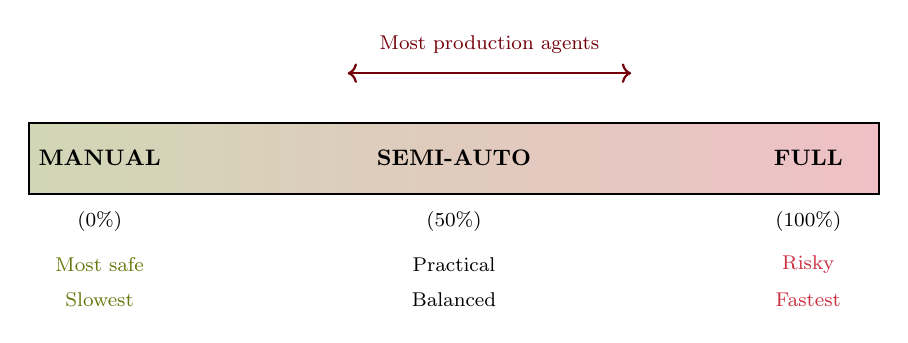
\begin{tikzpicture}[scale=0.9, transform shape]
        % Spectrum bar
        \fill[left color=UofSCHorseshoe!30, right color=UofSCRose!30] (-6, 0.5) rectangle (6, -0.5);
        \draw[thick, UofSCBlack] (-6, 0.5) rectangle (6, -0.5);

        % Labels on spectrum
        \node[font=\small\bfseries] at (-5, 0) {MANUAL};
        \node[font=\small\bfseries] at (0, 0) {SEMI-AUTO};
        \node[font=\small\bfseries] at (5, 0) {FULL};

        % Percentages
        \node[font=\footnotesize] at (-5, -0.9) {(0\%)};
        \node[font=\footnotesize] at (0, -0.9) {(50\%)};
        \node[font=\footnotesize] at (5, -0.9) {(100\%)};

        % Properties below
        \node[font=\footnotesize, text=UofSCHorseshoe] at (-5, -1.5) {Most safe};
        \node[font=\footnotesize] at (0, -1.5) {Practical};
        \node[font=\footnotesize, text=UofSCRose] at (5, -1.5) {Risky};

        \node[font=\footnotesize, text=UofSCHorseshoe] at (-5, -2) {Slowest};
        \node[font=\footnotesize] at (0, -2) {Balanced};
        \node[font=\footnotesize, text=UofSCRose] at (5, -2) {Fastest};

        % Arrow indicating typical range
        \draw[thick, UofSCGarnet, <->] (-1.5, 1.2) -- (2.5, 1.2);
        \node[font=\footnotesize, text=UofSCGarnet] at (0.5, 1.6) {Most production agents};
    \end{tikzpicture}
    \end{center}

    \vspace{0.5cm}
    \textbf{Why This Matters:}
    \begin{itemize}
        \item Higher autonomy = faster execution
        \item Lower autonomy = more control/safety
        \item Different tasks need different levels
    \end{itemize}

    \note{Autonomy is not a single setting but a design choice that affects the entire workflow. It's also not permanent---the same agent might operate at different autonomy levels for different tasks.}
\end{frame}

% --------------------------------------------
\begin{frame}{The Four Autonomy Levels}
    \begin{center}
    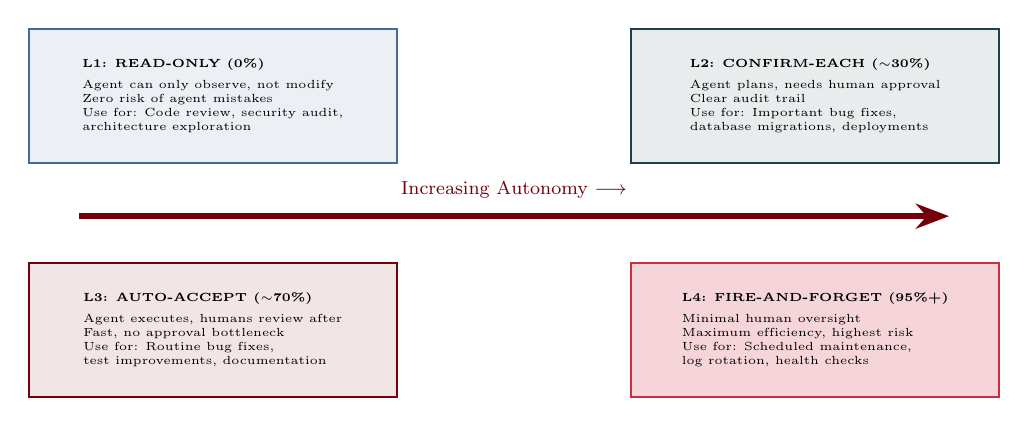
\begin{tikzpicture}[scale=0.85, transform shape]
        % L1
        \node[component atlantic, minimum width=5.5cm, minimum height=2cm, align=left, font=\tiny] (l1) at (-4.5, 2) {
            \textbf{L1: READ-ONLY (0\%)}\\[0.1cm]
            Agent can only observe, not modify\\
            Zero risk of agent mistakes\\
            Use for: Code review, security audit,\\
            architecture exploration
        };

        % L2
        \node[component congaree, minimum width=5.5cm, minimum height=2cm, align=left, font=\tiny] (l2) at (4.5, 2) {
            \textbf{L2: CONFIRM-EACH ($\sim$30\%)}\\[0.1cm]
            Agent plans, needs human approval\\
            Clear audit trail\\
            Use for: Important bug fixes,\\
            database migrations, deployments
        };

        % L3
        \node[component garnet, minimum width=5.5cm, minimum height=2cm, align=left, font=\tiny] (l3) at (-4.5, -1.5) {
            \textbf{L3: AUTO-ACCEPT ($\sim$70\%)}\\[0.1cm]
            Agent executes, humans review after\\
            Fast, no approval bottleneck\\
            Use for: Routine bug fixes,\\
            test improvements, documentation
        };

        % L4
        \node[component, fill=UofSCRose!20, draw=UofSCRose, minimum width=5.5cm, minimum height=2cm, align=left, font=\tiny] (l4) at (4.5, -1.5) {
            \textbf{L4: FIRE-AND-FORGET (95\%+)}\\[0.1cm]
            Minimal human oversight\\
            Maximum efficiency, highest risk\\
            Use for: Scheduled maintenance,\\
            log rotation, health checks
        };

        % Arrow showing progression
        \draw[arrow style, line width=2pt, UofSCGarnet] (-6.5, 0.2) -- (6.5, 0.2);
        \node[font=\footnotesize, text=UofSCGarnet] at (0, 0.6) {Increasing Autonomy $\longrightarrow$};
    \end{tikzpicture}
    \end{center}

    \note{Most production agents operate in the L2--L3 range. L4 is rare for important systems. L1 is used for exploration and review.}
\end{frame}

% --------------------------------------------
\begin{frame}{Choosing the Right Autonomy Level}
    \begin{columns}[T]
        \begin{column}{0.5\textwidth}
            \textbf{Key Questions:}
            \begin{enumerate}
                \item \textbf{What's the cost of failure?}\\
                Low cost $\rightarrow$ Higher autonomy

                \item \textbf{Can we detect failure?}\\
                Easy detection $\rightarrow$ Higher autonomy

                \item \textbf{Can we recover quickly?}\\
                Easy recovery $\rightarrow$ Higher autonomy

                \item \textbf{Do we trust the agent?}\\
                High trust $\rightarrow$ Higher autonomy
            \end{enumerate}
        \end{column}
        \begin{column}{0.5\textwidth}
            \begin{block}{Selection Guide}
                \footnotesize
                \begin{tabular}{ll}
                    \textbf{Task Type} & \textbf{Level} \\
                    \midrule
                    Security fixes & L2 \\
                    Performance bugs & L3 \\
                    Documentation & L3 \\
                    Test generation & L3 \\
                    Code review & L1 \\
                    Deployments & L2 \\
                    Exploration & L1 \\
                    Maintenance & L4 \\
                \end{tabular}
            \end{block}
        \end{column}
    \end{columns}

    \vspace{0.3cm}
    \begin{alertblock}{Best Practice}
        Start conservative, increase over time. Different agents at different levels. Match autonomy to task risk.
    \end{alertblock}

    \note{There's no universal answer---it depends entirely on the task and organization's risk tolerance.}
\end{frame}

% --------------------------------------------
\begin{frame}{Real-World Project: Mixed Autonomy Levels}
    \begin{center}
    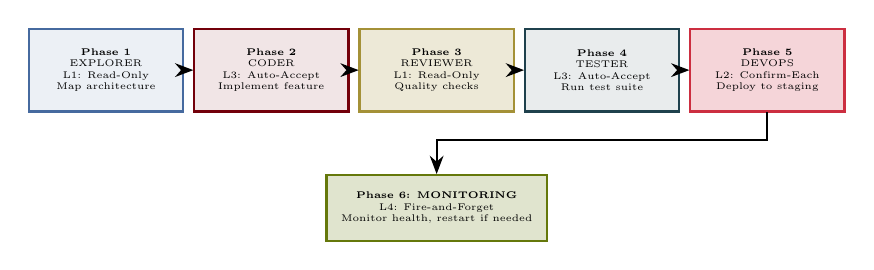
\begin{tikzpicture}[scale=0.7, transform shape]
        % Phases as a pipeline
        \node[component atlantic, minimum width=2.8cm, minimum height=1.5cm, font=\tiny, align=center] (p1) at (-6, 0) {
            \textbf{Phase 1}\\
            EXPLORER\\
            L1: Read-Only\\
            Map architecture
        };

        \node[component garnet, minimum width=2.8cm, minimum height=1.5cm, font=\tiny, align=center] (p2) at (-3, 0) {
            \textbf{Phase 2}\\
            CODER\\
            L3: Auto-Accept\\
            Implement feature
        };

        \node[component, fill=UofSCHoneycomb!20, draw=UofSCHoneycomb, minimum width=2.8cm, minimum height=1.5cm, font=\tiny, align=center] (p3) at (0, 0) {
            \textbf{Phase 3}\\
            REVIEWER\\
            L1: Read-Only\\
            Quality checks
        };

        \node[component congaree, minimum width=2.8cm, minimum height=1.5cm, font=\tiny, align=center] (p4) at (3, 0) {
            \textbf{Phase 4}\\
            TESTER\\
            L3: Auto-Accept\\
            Run test suite
        };

        \node[component, fill=UofSCRose!20, draw=UofSCRose, minimum width=2.8cm, minimum height=1.5cm, font=\tiny, align=center] (p5) at (6, 0) {
            \textbf{Phase 5}\\
            DEVOPS\\
            L2: Confirm-Each\\
            Deploy to staging
        };

        % Arrows
        \draw[arrow style] (p1) -- (p2);
        \draw[arrow style] (p2) -- (p3);
        \draw[arrow style] (p3) -- (p4);
        \draw[arrow style] (p4) -- (p5);

        % Monitoring below
        \node[component, fill=UofSCHorseshoe!20, draw=UofSCHorseshoe, minimum width=4cm, minimum height=1.2cm, font=\tiny, align=center] (p6) at (0, -2.5) {
            \textbf{Phase 6: MONITORING}\\
            L4: Fire-and-Forget\\
            Monitor health, restart if needed
        };

        \draw[arrow style] (p5.south) -- ++(0,-0.5) -| (p6.north);
    \end{tikzpicture}
    \end{center}

    \vspace{0.3cm}
    \textbf{Pattern:} Different agents at different levels in a coordinated pipeline

    \note{This shows how autonomy decisions aren't one-time but evolve throughout the system. The same organization uses L1 for critical review decisions but L4 for routine maintenance.}
\end{frame}

% ============================================
% CONCLUSION
% ============================================
\section{Summary \& Key Takeaways}

% --------------------------------------------
\begin{frame}{Part 2 Complete: Agent Foundations}
    \begin{columns}[T]
        \begin{column}{0.5\textwidth}
            \textbf{What We Covered:}
            \begin{itemize}
                \item \textbf{Section 1:} What IS an Agent?
                \begin{itemize}
                    \footnotesize
                    \item Formal definition
                    \item Agent vs traditional AI
                    \item Key characteristics
                \end{itemize}

                \item \textbf{Section 2:} Core Components
                \begin{itemize}
                    \footnotesize
                    \item LLM (Brain)
                    \item Memory/Context (Workspace)
                    \item Tools (Hands)
                    \item Planning
                \end{itemize}

                \item \textbf{Section 3:} The ReAct Loop
                \begin{itemize}
                    \footnotesize
                    \item REASON $\rightarrow$ ACT $\rightarrow$ OBSERVE
                    \item Why it works
                \end{itemize}
            \end{itemize}
        \end{column}
        \begin{column}{0.5\textwidth}
            \begin{itemize}
                \item \textbf{Section 4:} Agent Specialization
                \begin{itemize}
                    \footnotesize
                    \item Specialists vs Generalists
                    \item Common agent types
                    \item Design principles
                \end{itemize}

                \item \textbf{Section 5:} Context Windows
                \begin{itemize}
                    \footnotesize
                    \item Token arithmetic
                    \item Theory vs practice
                    \item Management strategies
                \end{itemize}

                \item \textbf{Section 6:} Autonomy Levels
                \begin{itemize}
                    \footnotesize
                    \item L1 through L4
                    \item Choosing the right level
                    \item Real-world mixing
                \end{itemize}
            \end{itemize}
        \end{column}
    \end{columns}

    \note{Recap all major themes. Students should leave this part with a solid understanding of what agents are, how they work internally, and how to design them effectively.}
\end{frame}

% --------------------------------------------
\begin{frame}{Foundational Principles}
    \begin{block}{The Five Core Principles}
        \begin{enumerate}
            \item \textbf{Agents are iterative, not one-shot}\\
            The ReAct loop: REASON $\rightarrow$ ACT $\rightarrow$ OBSERVE $\rightarrow$ repeat

            \item \textbf{Specialization beats generalization}\\
            Multiple focused agents $>$ One generalist agent

            \item \textbf{Context is finite and expensive}\\
            50\% for setup, 50\% for work; manage strategically

            \item \textbf{Autonomy must match task risk}\\
            Start conservative, increase as trust builds

            \item \textbf{Tools determine capability}\\
            Well-designed tools = effective agents; 8--15 is optimal
        \end{enumerate}
    \end{block}

    \vspace{0.3cm}
    \begin{center}
        \textcolor{UofSCGarnet}{\Large Agent Capability = LLM Quality $\times$ Tool Design $\times$ Memory Management $\times$ Planning}
    \end{center}

    \note{These are the key insights students should take away. Everything else builds on these principles.}
\end{frame}

% --------------------------------------------
\begin{frame}{Self-Check: Can You Explain...}
    \begin{enumerate}
        \item \textbf{To a non-technical person:}\\
        What an agent is and why it's different from ChatGPT?

        \item \textbf{Walk through a ReAct loop for ``fix this bug'':}\\
        What happens in REASON, ACT, OBSERVE?

        \item \textbf{Design a specialist agent for writing unit tests:}\\
        What tools would it have? What would it NOT have?

        \item \textbf{You have a 200K token context, project needs 30K tokens:}\\
        How would you manage this?

        \item \textbf{A task could be done at L2 or L3:}\\
        What questions would you ask to decide?
    \end{enumerate}

    \vspace{0.5cm}
    \begin{alertblock}{}
        \centering
        If you can answer these, you understand Part 2.
    \end{alertblock}

    \note{These self-check questions are the real learning objectives. Students don't need to memorize definitions---they need to be able to reason about agent design using these concepts.}
\end{frame}

% --------------------------------------------
\begin{frame}{Coming Up Next...}
    \begin{center}
    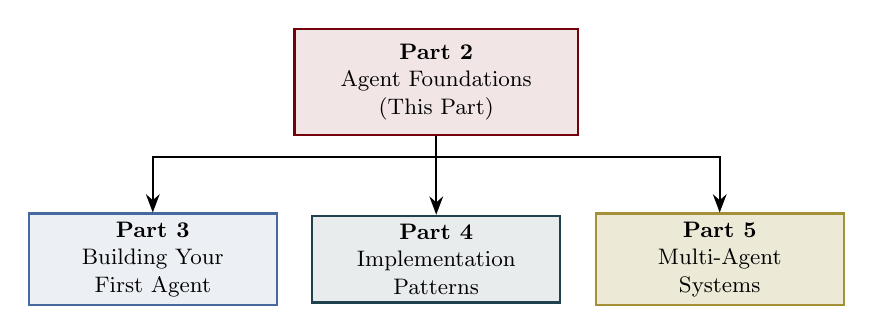
\begin{tikzpicture}[scale=0.9, transform shape]
        % Current part
        \node[component garnet, minimum width=4cm, minimum height=1.5cm] (current) at (0, 2) {
            \textbf{Part 2}\\
            Agent Foundations\\
            (This Part)
        };

        % Next parts
        \node[component atlantic, minimum width=3.5cm, minimum height=1.2cm] (p3) at (-4, -0.5) {
            \textbf{Part 3}\\
            Building Your\\
            First Agent
        };

        \node[component congaree, minimum width=3.5cm, minimum height=1.2cm] (p4) at (0, -0.5) {
            \textbf{Part 4}\\
            Implementation\\
            Patterns
        };

        \node[component, fill=UofSCHoneycomb!20, draw=UofSCHoneycomb, minimum width=3.5cm, minimum height=1.2cm] (p5) at (4, -0.5) {
            \textbf{Part 5}\\
            Multi-Agent\\
            Systems
        };

        % Arrows
        \draw[arrow style] (current.south) -- ++(0,-0.3) -| (p3.north);
        \draw[arrow style] (current.south) -- (p4.north);
        \draw[arrow style] (current.south) -- ++(0,-0.3) -| (p5.north);
    \end{tikzpicture}
    \end{center}

    \vspace{0.5cm}
    \textbf{From Theory to Practice:}
    \begin{itemize}
        \item Part 3: Implement your first Explorer + Coder agents
        \item Part 4: Common patterns (pipelines, parallel execution, feedback loops)
        \item Part 5: Agent communication, shared state, emergent behavior
    \end{itemize}

    \note{This frames Part 2 as foundational knowledge that will be applied immediately. Students should feel they now have the conceptual vocabulary and mental models needed.}
\end{frame}

% --------------------------------------------
\begin{frame}[plain]
    \begin{center}
        \vspace{2cm}
        {\Huge\textcolor{UofSCGarnet}{\textbf{Questions?}}}

        \vspace{1.5cm}
        {\Large Part 2: Agent Foundations \& Concepts}

        \vspace{0.5cm}
        {\large Agentic Coding Tools Series}

        \vspace{1.5cm}
        {\footnotesize University of South Carolina}
    \end{center}
\end{frame}

\end{document}
